\chapter{Theory}
\label{cha:theory}

This chapter introduces relevant theory and related work 

\section{Active Vision and Visual Search}

An \textit{active vision} system is a system that can manipulate the viewpoint of the camera in order to investigate the environment and get better information from it.



\section{Reinforcement Learning}

Reinforcement learning (RL) is a subfield of machine learning concerned intelligent agents that learn to achieve some goal through interaction with their environment. An agent is conditioned to improve its behaviour through reward and punishment. In this section, some key concepts will be introduced.

\subsection{Markov Decision Process}

The problem of learning from interaction to achieve a goal is usually framed as a (finite) Markov Decision Process (MDP). An \textit{agent} learns by interacting with an \textit{environment}. At each discrete time step \(t = 0, 1, 2, \dots\), the agent perceives some representation of the \textit{state} \(S_t\) of its environment. The agent selects some \textit{action} \(A_t\) to execute, and one timestep later receives a reward \(R_{t+1}\) as well as a representation of the new environment state \(S_{t+1}\). This continues until the final time step \(T\) which is the end of the \textit{episode}. The goal of the agent is to maximize the \textit{discounted return}, defined as \(G_t \doteq \sum_{k=t+1}^T \gamma^{k-t-1} R_{k}\) for some \(\gamma \in [0, 1]\) that reflects the uncertainty of the environment.   

In some cases the agent can not perceive the underlying state of the environment. Instead, at each time step \(t\) the agent perceives a partial \textit{observation} \(O_t\). The environment is assumed to have some well defined underlying \textit{latent state} that that is not available to the agent. Assuming that the underlying process dynamics are still determined by an MDP this is referred to as a partially observable Markov decision process (POMDP). A POMDP is formally defined as a 7-tuple \(\langle \mathcal{S}, \mathcal{A}, \mathcal{O}, \mathcal{R}, \mathcal{T}, \Omega, \gamma \rangle\), where

\begin{itemize}
    \item \(\mathcal{S} = \{ s_1, s_2, \dots, s_n \}\) is a set of states,
    \item \(\mathcal{A} = \{ a_1, a_2, \dots, a_m \}\) is a set of actions,
    \item \(\mathcal{O}\) is a set of conditional observation probabilities \(\mathcal{O}(o | s^\prime, a)\),
    \item \(\mathcal{R} : S \times A \rightarrow \mathbb{R}\) is a reward function,
    \item \(\mathcal{T}\) is a set of conditional state transition probabilities \(\mathcal{T}(s^\prime | s, a)\),
    \item \(\Omega = \{ o_1, o_2, \dots, o_k \}\) is a set of observations, and
    \item \(\gamma \in [0, 1]\) is a discount factor.
\end{itemize}

%An MDP satisfies the Markov property: the process is memoryless. A POMDP is not memoryless, as observations only convey part of the underlying state. However, the \textit{history} \(H_t = A_0, O_1, R_1, \dots, A_{t-1}, O_t, R_t\) does.

\begin{figure}
    \centering
    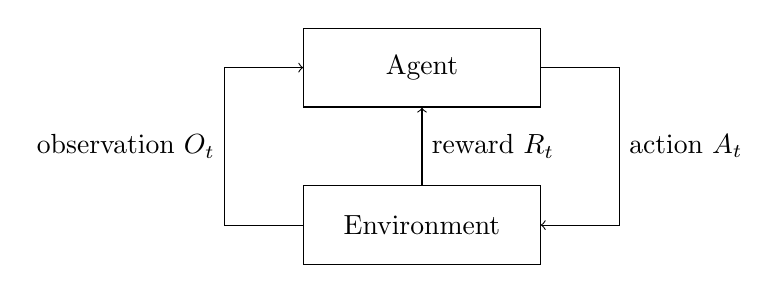
\begin{tikzpicture}[node distance=2cm]
        \tikzstyle{block} = [rectangle,minimum width=3cm,minimum height=1cm,text centered,draw=black,fill=white]
        \node (agent)[block]{Agent};
        \node (environment)[block,below of=agent]{Environment};
        \draw [->] (agent.east) -- ++(1cm,0) -- node [anchor=west]{action \(A_t\)} ++(0,-2cm) -- (environment.east);
        \draw [->] (environment.north) -- node [anchor=west]{reward \(R_t\)} (agent.south);
        \draw [->] (environment.west) -- ++(-1cm,0) -- node [anchor=east]{observation \(O_t\)} ++(0,+2cm) -- (agent.west);
    \end{tikzpicture}
    \label{fig:pomdp}
    \caption{Partially observable Markov decision process.}
\end{figure}

\subsection{Policies and Value Functions}

Most RL algoerithms estimate both a \textit{value function} that tells the agent how good it is to be in a given state, and a 

\subsection{Policy Optimization}

This work will focus on policy optimization algorithms.

\subsection{Taxonomy of Algorithms}

\begin{itemize}
    \item Model-free vs. model-based
    \item 
\end{itemize}

\subsection{Generalization}

% reality is dynamic
% agents need to be robust to variation
% capability to transfer and adapt to unseen but similar environments
% most current research works on benchmarks that do not test this (MuJoCo, Arcade learning environment)

% refer to survey
% specifically IID (train_dist = test_dist) and OOD environments (train_dist != test_dist)